
% this file is called up by thesis.tex
% content in this file will be fed into the main document

%: ----------------------- introduction file header -----------------------
\chapter{Conclusions and Future Work}\label{ch:conclusion}

\graphicspath{{conclusions/figures/}}

The main goal of the work presented in this thesis was to facilitate the exploration of large multilingual document corpora through the use of probabilistic topic models. To this end, we developed a framework that covers the full life-cycle of topic models, including their generation, publication and reuse. We have also created a representation model for documents where the main topics of a text are described through hierarchical annotations, and relations among documents are calculated based on a similarity metric optimized for large scale processing. Finally, we have developed unsupervised topic alignment techniques using conceptual representations of topic words to relate multilingual texts. 

Based on the evaluation of our results, we extract two main conclusions. The first one is that \textit{it is sufficient to use the most representative topics to relate texts, and hierarchical representation can be also used for this purpose}. However, an important finding is that \textit{not all topics have the same discriminatory capacity to relate texts}. Topics arise in a model to describe the content used from a training dataset. If the number of topics is not enough with respect to the diversity of content of the document collection, there will be too general topics that have a reduced discriminative capacity. For example, given a document collection where 50\% papers are focused on astronomy, 30\% on agriculture , 10\% on mathematics, 5\% on psychology and 5\% on pharmacy, if the topic model is created with only 3 topics, one will describe astronomy, another agriculture and the third will be a mixture of the other topics. This third topic distinguishes documents that do not deal with astronomy or agriculture, but does not distinguish between mathematics, psychology or pharmacy. It is a topic with a limited discriminative capacity.


The second conclusion is that \textit{conceptual representations of probabilistic topics can abstract the description of multilingual texts in a language-independent space hence allowing for usual tasks over multilingual corpora}. However, we have found that the relations in this space \textit{tend to generalize more than word-based representations}. 

The rest of the section discusses our assumptions and restrictions, contributions, impact, current limitations and future lines of work. 
% -------------------------------------------------------------
% -- Conclusion
% -------------------------------------------------------------

\section{Assumptions and Restrictions}

Throughout the thesis, we have considered a series of assumptions and restrictions for our work. Our first assumption is that \textit{probabilistic topic distributions allow to semantically relate texts} (A1).

Also, in order to apply successfully our framework to handle probabilistic topic models, we convert \textit{topic models to RESTful web services }(R1). We restrict to this type of services because it is the most common in web development and facilitates interoperability. 

Furthermore, we assume that \textit{all the most representative words of a probabilistic topic can be converted to concepts using cognitive synsets} (A2). These conceptual representations of topics allow relating them across languages. In addition, \textit{texts are grammatically valid} (A3) and \textit{syntactically correct} (A4). Phrases are well constructed and have no misspellings, so that nouns, adjectives and verbs can be correctly extracted to prepare the bag-of-words that train the topic models and characterize the texts. 

Finally, our last assumption is that, \textit{the categorization of texts and the association of related texts facilitates the exploration of large documentary corpora.} (A5).

Tables \ref{table:assumptions} and \ref{table:rectrictions} summarize our assumptions and restrictions according to their description.

\begin{table}[!htbp]
\begin{tabularx}{\linewidth}{Sb}
\toprule
\heading{Assumption} & \heading{Description} \\
\midrule
\midrule
A1 & Probabilistic topic distributions allow to semantically relate texts\\
\midrule
A2 & Words can be converted to concepts using cognitive synsets\\
\midrule
A3 & Texts are grammatically valid\\
\midrule
A4 & Texts are syntactically correct\\
\midrule
A5 & Text categorization and association facilitates the exploration of large corpora\\
\bottomrule
\end{tabularx}
\caption{Assumptions considered in this thesis.}
\label{table:assumptions}
\end{table}

\begin{table}[!htbp]
\centering%
\begin{tabularx}{\linewidth}{Sb}
\toprule
\heading{Restriction} & \heading{Description} \\
\midrule
\midrule
R1 & Topic models are distributed as RESTful web services\\
\bottomrule
\end{tabularx}
\caption{Restrictions considered in this thesis.}
\label{table:rectrictions}
\end{table}

\section{A Summary of Our Contributions}

In this section we summarize our contributions regarding the research challenges defined on Chapter \ref{ch:hypothesis}.


\subsection{Topic Model Distribution}
Our main contributions to this research challenge are the librAIry framework (addressing partly RCInterface1, \textit{reuse of topic models is limited by incompatibility problems}), and a methodology for publishing probabilistic topic models as web services (addressing RCInterface2, \textit{there is no standard that unifies the representation of topic models}).

\subsubsection{librAIry Framework}

In Chapter \ref{ch:scalability} we described our framework to cover the entire topic model life-cycle in a scalable way. librAIry is a modular system that processes and analyzes huge collections of textual resources creating and using probabilistic topic models. It has been designed to represent corpora by organizing data at: \textit{snippets} to reflect piece of texts, \textit{documents} to represent full texts, and \textit{domains} to group documents. Transversally there are \textit{annotations}, which allow providing more details to any of them.

There are four types of modules involved in processing the resources: harvester, annotator, modeler and admin. They are based on the SEDA principles, where actions over resources and status change notification events are introduced to distribute the operations. \textit{Harvester} modules create new \textit{documents}, \textit{snippets} and \textit{domains}. \textit{Annotator} modules react to each new resource and create \textit{annotations}. \textit{Modeler} modules create new topic models from a \textit{domain}. And \textit{admin} modules perform administrative tasks.

The librAIry framework has evolved since its creation, and has been tested as part of the Corpus Viewer platform \citep{Samy2019}, where it was used to analyze the current situation and trends of information and communication technologies (ICT) through the study of patent collections and grants for R\&D projects (see Section \ref{sec:corpus-viewer}). We have also used this implementation to support complex calculations on data sets that were not necessarily text. For example, to relate patients according to the medicines they receive \citep{Badenes-Olmedo2019c} (see Section 	\ref{sec:polypharmacy}), or to relate medicines or diseases from the experiments where they are used (see Section \ref{sec:drugs4covid}).

\subsubsection{Method for publishing topic models as Web Services}

Our second contribution consists of a method to make topic models openly accessible as web resources. Our proposal is to publish probabilistic topic models following a RESTful API paradigm. This allows easy accessibility and reuse for both humans and machines aiming to consume topic model related information.

As described in Section \ref{sec:topic-model-publication} three tasks guide the creation of a topic model as web service: \textit{reproducibility}, \textit{exploration} and \textit{inference}. A list of available methods for using a topic model is provided in Table \ref{table:operations}. In order to facilitate the reuse of the topic models published as web service, section \ref{sec:topic-model-exploitation} presents an online repository based on virtual services.

\subsection{Explainable Topic-based Similarity}

Understanding the relations between texts from density-based metrics that measure the differences between probabilistic topic distributions is not simple. We have made two main contributions in this thesis to alleviate that difficulty: a method to identify the most relevant topics regardless of the dimensions of the model, addressing RCExplainable-1 (\textit{there is no common criteria for identifying the most representative topics in a document}, and a distance metric based on the most relevant topics that relates similar texts, addresing RCExplainable2 (\textit{it is difficult to understand the distance between topic distributions}) and RCExplainable3 (\textit{there is no common criterion for determining wheter documents are related}).

\subsubsection{Most Relevant Topics}

In Section \ref{sec:topic-relations}, we explored the ability of topics to describe scientific articles and concluded that texts with greater vocabulary, that emphasize key terms through repetition, favor topic-based representation. 

Taking into account the relevance of topics to describe texts, we analyzed the behavior of topic distributions when using topic models with different dimensions, i.e. different number of topics. After our evaluations we saw that the most relevant topics cannot be identified by fixed thresholds, since as the dimensions of the model vary the relative weights also vary. Nor can they be identified using clustering techniques based on centroids, since the number of groups with homogeneous weights is unknown a priori. With these results, we proposed a technique to identify relevant topics based on density clustering, so that each level of relevance groups topics with similar relative weights.

\subsubsection{Distance Metric based on Topic Relevance}

A method of relating documents from their most representative topics was proposed in Section \ref{sec:topic-clustering}. It is based on a distance metric that takes advantage of representations only based on the most relevant topics to describe texts. The distance between two texts is proportional to the number of topics they share at the same relevance levels.

The performance of the metric was evaluated by automatically clustering the JRC-Acquis corpus according to EUROVOC categories. Tables \ref{tab:precisionHe}, \ref{tab:precisionJS}, \ref{tab:recallHe} and \ref{tab:recallJS} show promising results with high precision and recall in unsupervised classification tasks.


\subsection{Data Structures and Algorithms for Large-Scale Comparisons of Documents}

Brute-force techniques cannot be applied to compare all items in a huge corpus. Our two main contributions to this research challenge are a data structure to describe documents from their most relevant topics, that partially addresses the RCComparison1 (\textit{there are no mechanisms that efficiently partition the topic-based search space without compromising the ability for thematic exploration}), and an efficient algorithm to make comparisons on a large scale based on topic relevance, that addresses RCComparison2 (\textit{there are no similarity metrics that compare partial distributions of topics}).

\subsubsection{Topic Hierarchies Representation}

We created a new data structure to represent topic distributions as topic hierarchies that uses the relevance of each topic to define hierarchy levels. This way of encoding documents has also helped to understand why two documents are similar, based on the intersection of topics at hierarchies of relevance.

The approach can accommodate additional query restrictions when searching for related documents (e.g. documents that mainly deal with one theme, although they also deal with another) and has proven to obtain high-precision results. 

\subsubsection{Comparisons based on Topic Hierarchies}

With large amounts of items in a collection, discovering the entire set of nearest neighbors to a given document is infeasible. Due to the low storage cost and fast retrieval speed, hashing is one the popular solutions for approximate nearest neighbours. However, existing hashing methods for probability distributions only focus on the efficiency of searches from a given document, without handling complex queries or offering hints about why one document is considered more similar than another.

We developed a method to compare and organize huge document collections based on similar topic hierarchies. The hierarchy levels are compared and the distance between texts depends on the degree of intersection between pair of representations.

In addition, the technique to represent and compare documents has been implemented in our librAIry framework.

\subsection{Multilingual Corpora}

Document in different languages must be described by multilingual topics to be thematically related without having to translate their texts. However, parallel or comparable corpora, or multilingual dictionaries are required to abstract topics into a language-independent space. Our main contribution to this research challenge is a method that automatically creates a topic-based space shared among all languages from the language-dependent models independently created. It address the RCCrossLingual1 (\textit{there are no approaches to abstract probabilistic topics in language-independent spaces without translating text or aligning documents}) 

\subsubsection{Cross-lingual Topics}

We proposed a unique space to describe documents based on topic models created from different languages. Topics are created independently for each language, and are projected on concepts instead of words. On concept-based representations, documents in different languages coexist together and can be related.

Representations are analyzed in classification and information retrieval tasks on multilingual document collections. As expected, the performance in terms of accuracy is not as good as that of the approach based on prior knowledge (i.e. topics previously aligned by documents annotated with categories). However, in terms of coverage, the performance of the unsupervised approach is much greater than that offered by the semi-supervised approach, to the point of offering better overall performance (i.e f1) in classification tasks. 

In addition, the algorithm proved to perform close to the semi-supervised algorithm in information retrieval task, which makes us think that the process of topic annotation by set of synonyms (i.e. concepts) can be improved to filter those elements that are not sufficiently representative.


\section{Impact}

The contributions of this thesis have already started to be used in recent work by other researchers. The librAIry framework was used, among others, to create, publish, distribute and reuse probabilistic topic models for studing the Language Technologies (TL) sector in Spain \citep{Samy2019}. The analysis took into account  the structured and unstructured data from the ACL Anthology repository in order to portray the current panorama in terms of underlying topics and their evolution in recent years in comparison with the international community. The framework has also been used to facilitate the classification of public offering using big data techniques \citep{Olga2019} and to analyze texts in reading support systems \citep{Teresa2020}.

Our methods to categorize documents through topic hierarchies and to make efficient large-scale comparisons  have been adapted to other domains. In \citep{Badenes-Olmedo2019c} they were adapted to compare patients from representations based on the medications they were using. The approach is very similar since drugs, like topics, can be distributed in different proportions according to the patient. To take advantage of the hierarchical representation of the topics, a more complex approach based on drug-drug interactions was performed (see Section \ref{sec:polypharmacy}).

Other contributions may impact different research areas, as we describe below:
\begin{itemize}
\item \textbf{Corpus Exploration}: By knowing how topics are present in a corpus in terms of relevance, it is possible to derive a thematic network where the nodes represent the different topics and the edges are the documents containing them on the same level of relevance. Thus, the higher the number of common documents the stronger the connection would be between two topics. This kind of network would help users to see how different topics are connected with each other in a corpus, facilitating the exploration between topics.
\item \textbf{Topic Discovery}: Commonly occurring topics, when supported in many documents, may become valuable topic candidates themselves. Documentary management system may offer these potentially new topics to users to include in their corpus description.
\item \textbf{Language Abstraction}: Approaches like \citep{hao-paul-2018-learning} create multilingual topics from incomparable corpora. These approaches can benefit from our hierarchical representations to create language-independent spaces where documents are described by their most relevant topics.
\item \textbf{Corpus Visualization}: As stated in Section \ref{ch:comparisons}, one of the reasons why groupings are created is for summarization and organization purposes. Hence, commonly occurring topics by hierarchies can be used to simplify the complexity of a corpus by collapsing their documents under a single group. If a corpus has overlapping clusters it would be possible to create different views according to user preferences, simplifying the overall complexity shown to the final user.
\item \textbf{Corpus Compression}: Similarly, if several documents share the same most relevant topics, it would be possible to store the common relevant topics instead of every unique topic distribution, for efficiency. This would be particularly useful when dealing with similar or identical texts.
\item \textbf{Topic Suggestions}: Commonly relevant topics may be used to suggest how a user may complete the writing of a document. By comparing the current topic hierarchies with the commonly relevant topics, it would be possible to recommend the next topic o topics to be considered in the document.
\item \textbf{Document Ranking}: Once the topics are described by hierarchies of relevance, it would be possible to order the documents in a corpus by different criteria and create rankings. Possible examples of rankings are basic searches based on one or several highly relevant topics, or more complex searches that combine different topics and different degrees of relevance.  
\end{itemize}

%\section{Limitations}
%...

\section{Future Work}

Our work may be expanded in several ways. In this section we discuss possible future lines of work related to our research challenges.

\begin{itemize}
\item \textbf{Extend the Reuse of Topic Models}: There are several ways in which our topic services may be improved to be more useful. First, it would be necessary to study the different tasks where a topic model can be used in order to allow users to customize their inferences. As we have seen in our analysis, classification and information retrieval tasks require topic distributions as vectors of weights and also as hierarchies of relevance, as well as having the weights of the words for each topic. Other metadata like the corpus used to train it, accessible and downloadable, or the libraries used to create the model may be relevant for facilitate reproducibility and improvement of existing models.

Second, it should be possible to rank topic models once they have been created and distributed. Rankings make a set of topic models easily comparable in order to recommend similar topic models to a particular task (based on the same training set or similar categories). It would be an interesting line of work to determine if a recommendation based on similar topic models provides similar or better results than other approaches to solve the same problems.

Third, a set of topic models may be used for suggestions in corpus exploration, in combination with text mining approaches. Text mining approaches have been demonstrated to obtain good results to classify o retrieve texts from a corpus. When using text mining techniques with topic models as services, we suspect that good results may be obtained, as context information can be added using categories from these topics. 
\item \textbf{Combined Representation of Topic Models}: There are many of scenarios where big collections of documents, sometimes available in different languages, have to be browsed according to certain priorities/information needs, e.g. in the medical domain huge amounts of medical reports are daily created offering the possibility of extracting knowledge from them. How they can be explored and effectively consumed will depend on the medical specialty considered. 

Psychiatrists may be looking for collections of reports related by the patient\'s mood, while pharmacists may want to find patients with the same adverse reactions. In a first approach, only structured information are considered (e.g disease, patient, location, date, insurance). This limits the ability to relate reports with information not described by keywords or that cannot be matched because it is written in different languages (e.g. patient mood, response to medications, or behavior during treatment). 

In such situations it would be advantageous to be able to rely on language-agnostic and unsupervised annotation units derived from the text so the full content does not need to be translated, for instance by inferring the notion of topics discussed in the documents. In this research line, probabilistic topic models can open the door to a new set of possibilities to automatically learn cross-lingual concepts to browse multi-lingual medical report collections. Thanks to these techniques, patients who, having different illnesses, manifest similar behaviors from a particular point of view can thus be related (Figure \ref{fig:context-similarity}). 

The greater the presence or absence of concepts is leading the final similarity score, but it might be an oversimplification of what this approach is really doing as it can be based on topic hierarchies. Diagnoses could therefore be supported by collections of similar medical reports from multiple medical areas, in different languages, and in real-time. Thanks to approaches like this one, a pharmacist in Paris could find patients in India who have similar reactions without medication, described in their reports, to those detected when certain medications are prescribed. Similarly, a German psychiatrist is able to check how some pregnant women in England share similar symptoms to patients with anxiety problems after having heart surgery.
\item \textbf{Refine the Conceptual Abstractions of Topics}:In this thesis we have proposed a way of creating language-independent abstractions of probabilistic topics: representations based on concepts, instead of words, created by cognitive synonyms (i.e. synsets). Even though we have contributed towards the automatic alignment of multilingual topics, our work may be expanded, as we further describe below. 

As demonstrated in evaluations on document retrieval and classification tasks, the accuracy of our approach is reduced because concepts are more general than words to describe topics. The mapping between words and concepts to describe a topic should be reviewed to create representations that are general enough to relate topics from different languages, and precise enough to separate different topics. 

\end{itemize}


\begin{figure}[ht]
    \centering
    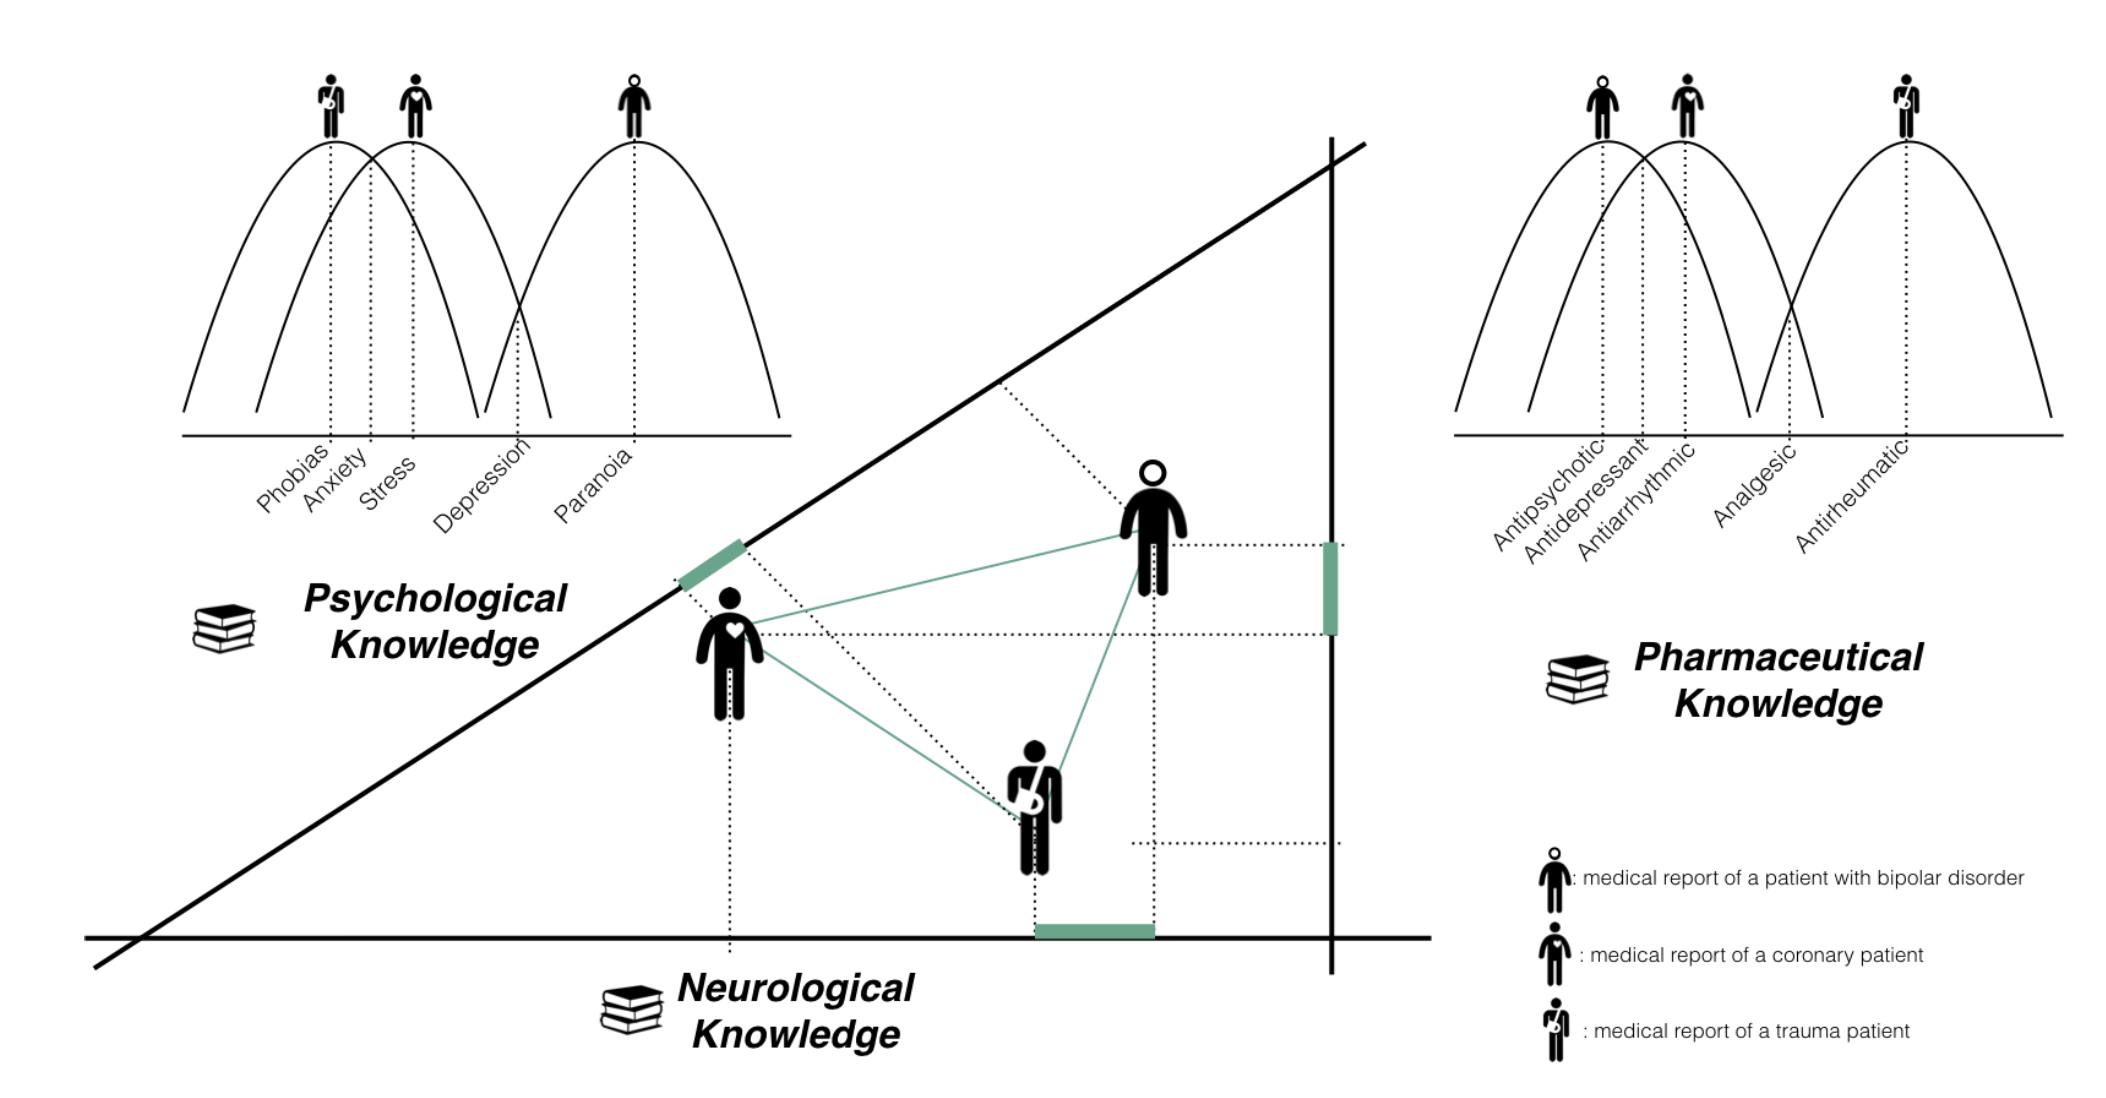
\includegraphics[width=0.7\linewidth]{context-similarity.png}
    \caption{Similarity among medical reports depends on the reference knowledge used to analyze them}
    \label{fig:context-similarity}
\end{figure}


